	\newpage
\section{Implementacja}		%4
%Wkleić szkielet kodu, wraz z komentarzami. Opisać zmienne, struktury do czego służą. Opisać procedury, metody co wykonują. Opisać nowe zdefiniowane klasy. Opisać dziedziczenie. Opisać nowo utworzone pliki za co odpowiadają.
\subsection{Pierwsze kroki}
\textit
{
	Po stworzeniu projektu poznawaliśmy strukturę oraz działanie aplikacji próbując modyfikować istniejące już klasy. Po zapoznaniu się z podstawami realizowaliśmy dalsze tutoriale aby 			swobodnie pracować w środowisku Xamarin'a.
}

\subsection{Modyfikacja menu}

\textit
{
	Pierwszym zadaniem było ustalenie szaty graficznej, widoku podstawowego z przyciskiem oraz menu. Aby to zrobić należało wykonać następujące czynności:\\\\
	-Dopisać odpowiednie właściwości do kodu XML typu background color, font-size, padding, textcolor itp. aby wystylizować układ widoku.\\\\
	Fragment modyfikacji:
	\begin{figure}[!htb]
		\begin{center}
			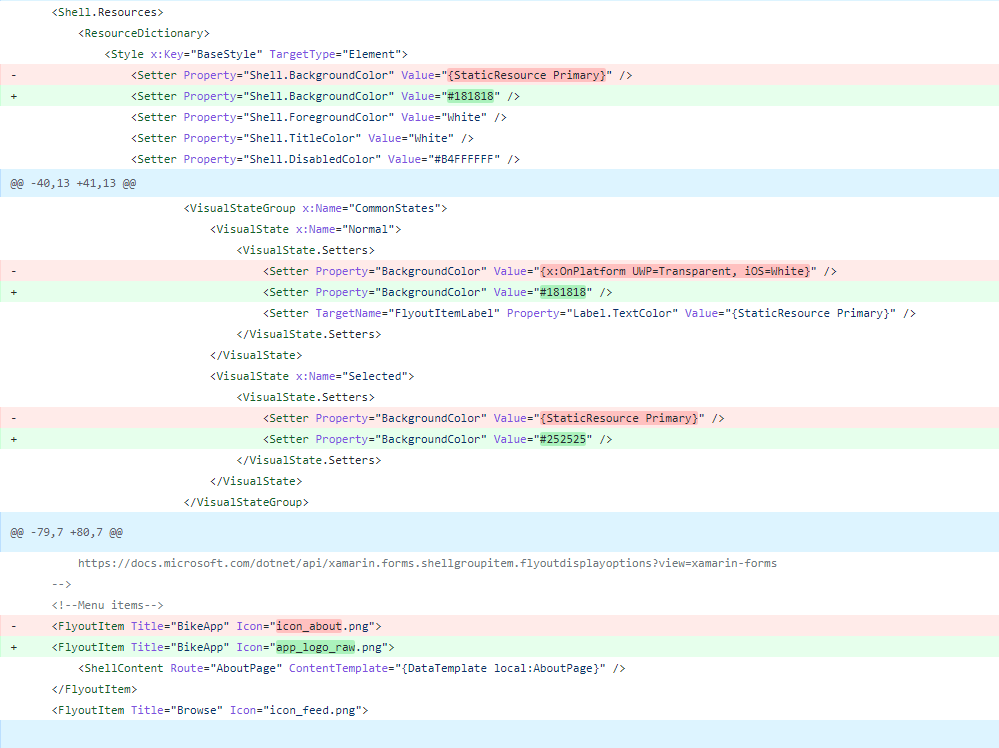
\includegraphics[width=15cm]{rys/gitchanges1.png}
			\caption{Zmiany styli}
			\label{rys:Zmiany styli}
		\end{center}
	\end{figure}
}

\newpage
\textit
{
	-Stworzyć widok główny na podstawie języka XML oraz metody w języku C\# informującej o kliknięciu w przycisk.\\\\
	Fragment modyfikacji:
	\begin{figure}[!htb]
		\begin{center}
			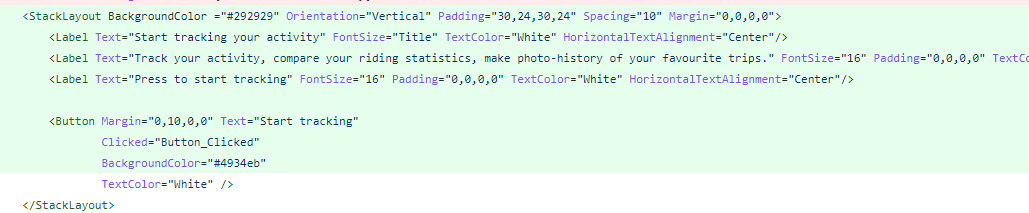
\includegraphics[width=15cm]{rys/gitchanges2.png}
			\caption{Implementacja widoku}
			\label{rys:Implementacja widoku}
		\end{center}
	\end{figure}
}

\textit
{
	-Pobrać i zainstalować paczkę 'acr' z nuget packages, zaimplementować opcję alertu, zaktualizować wersję xamarin.forms z 5.0.0.2012 do 5.0.0.2125 z powodu konfliktu biblioteki 				emulującej android w języku java \\\\
	Zmiany widoczne w kodzie:
	\begin{figure}[!htb]
		\begin{center}
			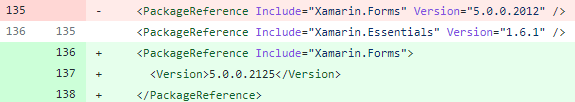
\includegraphics[width=15cm]{rys/gitchanges3.png}
			\caption{Modyfikacja nuget packages}
			\label{rys:Modyfikacja nuget packages}
		\end{center}
	\end{figure}
}

\newpage
\subsection{Dodanie oraz wystylizowanie elementów menu}

\textit
{
	Na początku należało utworzyć odpowiednie widoki aby stworzyć spójny szkielet aplikacji \\
	\begin{figure}[!htb]
		\begin{center}
			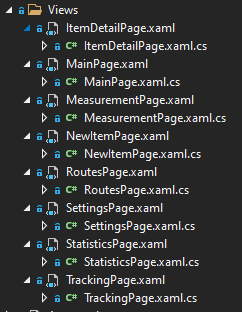
\includegraphics[width=7.5cm]{rys/gitchanges4.2.1.png}
			\caption{Szkielet widoków}
			\label{rys:Szkielet widoków}
		\end{center}
	\end{figure}
}

\textit
{\\
	Następnie należało stworzyć odpowiadające im modele widoków\\
	\begin{figure}[!htb]
		\begin{center}
			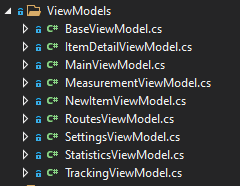
\includegraphics[width=7.5cm]{rys/gitchanges4.2.2.png}
			\caption{Szkielet modeli widoków}
			\label{rys:Szkielet modeli widoków}
		\end{center}
	\end{figure}
}

\newpage
\textit
{
	Potem należało ustawić odpowiednie parametry tak aby połączyć poszczególny widok z jego modelem\\
	\begin{figure}[!htb]
		\begin{center}
			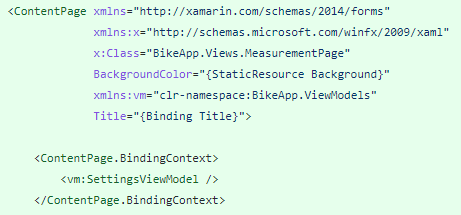
\includegraphics[width=15cm]{rys/gitchanges4.2.3.png}
			\caption{Binding ModelView z View}
			\label{rys:Binding ModelView z View}
		\end{center}
	\end{figure}
}

\newpage
\textit
{
	Kolejnym krokiem było ustawienie odpowiednich opcji flyoutmenu:\\
	\begin{figure}[!htb]
		\begin{center}
			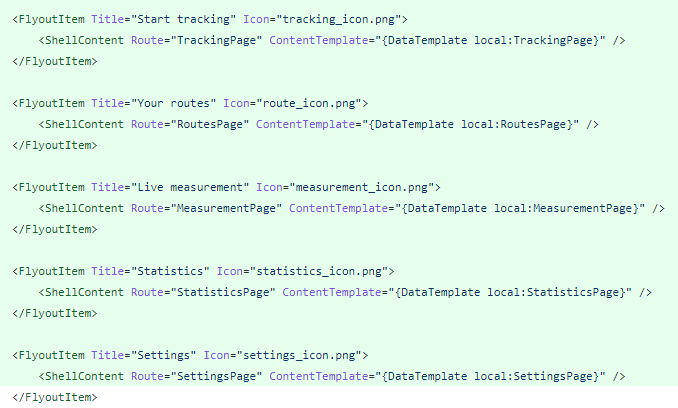
\includegraphics[width=15cm]{rys/gitchanges4.2.4.png}
			\caption{Dodanie opcji menu}
			\label{rys:Dodanie opcji menu}
		\end{center}
	\end{figure}
}

\newpage
\textit
{
	Po zakończeniu należało stworzyć oraz dodać odpowiednie ikony wraz z tytułami do każdego widoku\\
	\begin{figure}[!htb]
		\begin{center}
			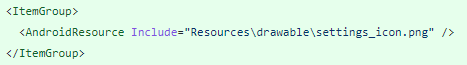
\includegraphics[width=15cm]{rys/gitchanges4.2.5.png}
			\caption{Dodanie styli}
			\label{rys:Dodanie styli}
		\end{center}
	\end{figure}
	\begin{figure}[!htb]
		\begin{center}
			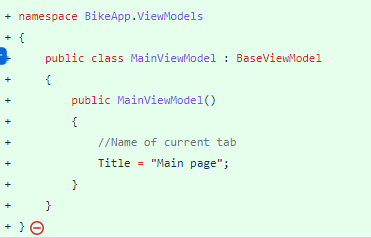
\includegraphics[width=10cm]{rys/gitchanges4.2.6.png}
			\caption{Dodanie styli}
			\label{rys:Dodanie styli}
		\end{center}
	\end{figure}
	\begin{figure}[!htb]
		\begin{center}
			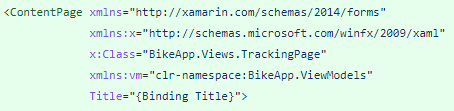
\includegraphics[width=15cm]{rys/gitchanges4.2.7.png}
			\caption{Dodanie styli}
			\label{rys:Dodanie styli}
		\end{center}
	\end{figure}
}

\newpage
\textit
{
	Na koniec należało wszystko wystylizować oraz poprawić ewentualne błędy w kodzie\\
	\begin{figure}[!htb]
		\begin{center}
			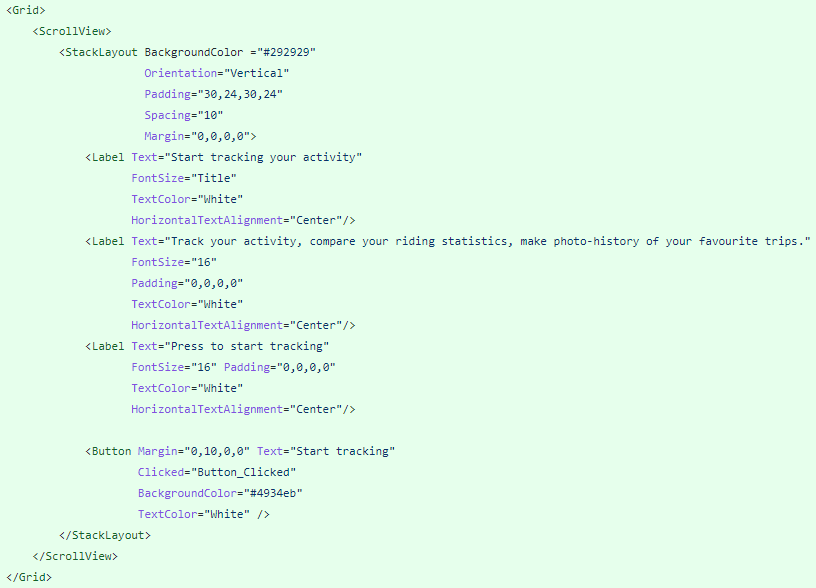
\includegraphics[width=15cm]{rys/gitchanges4.2.8.png}
			\caption{Finalizacja}
			\label{rys:Finalizacja}
		\end{center}
	\end{figure}
}

\newpage
\textit
{
	Efekt finalny:\\
	\begin{figure}[!htb]
		\begin{center}
			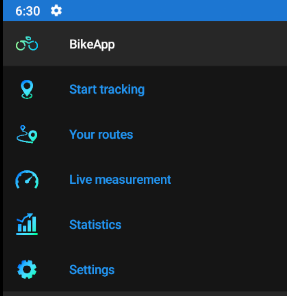
\includegraphics[width=10cm]{rys/gitchanges4.2.9.png}
			\caption{Finalizacja}
			\label{rys:Finalizacja}
		\end{center}
	\end{figure}
}

\newpage
\subsection{Dodanie motywu jasnego i ciemnego}

\textit
{
	Na początku należało utworzyć odpowiednie klasy przechowujące kolory \\
	\begin{figure}[!htb]
		\begin{center}
			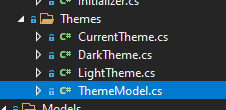
\includegraphics[width=7.5cm]{rys/gitchanges4.2.10.png}
			\caption{Układ klas}
			\label{rys:Układ klas}
		\end{center}
	\end{figure}
	\begin{figure}[!htb]
		\begin{center}
			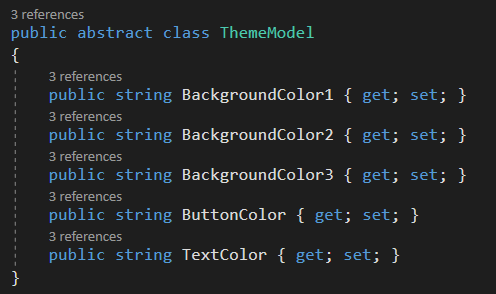
\includegraphics[width=10cm]{rys/gitchanges4.2.11.png}
			\caption{Abstrakcyjna klasa bazowa}
			\label{rys:Abstrakcyjna klasa bazowa}
		\end{center}
	\end{figure}
	\begin{figure}[!htb]
		\begin{center}
			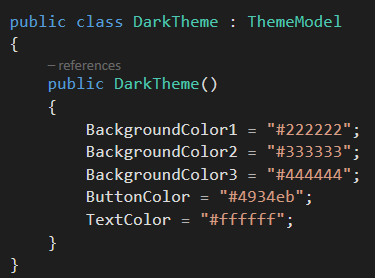
\includegraphics[width=10cm]{rys/gitchanges4.2.12.png}
			\caption{Przykładowy motyw dziedziczący po klasie bazowej}
			\label{rys:Przykładowy motyw}
		\end{center}
	\end{figure}
	\begin{figure}[!htb]
		\begin{center}
			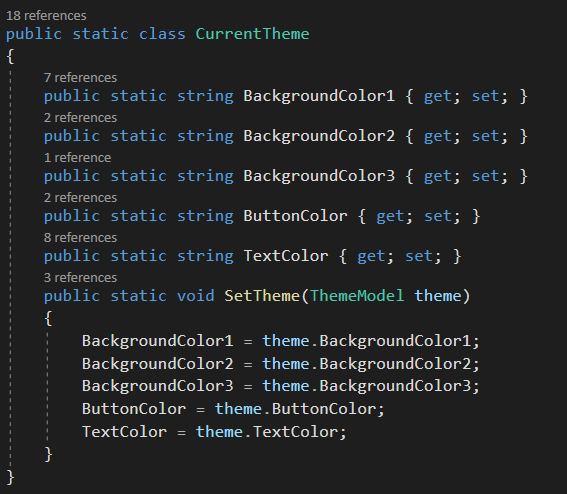
\includegraphics[width=10cm]{rys/gitchanges4.2.13.png}
			\caption{Klasa przechowująća aktualny motyw ustawiana na podstawie modelu abstrakcyjnego}
			\label{rys:Klasa przechowująca aktualny motyw}
		\end{center}
	\end{figure}
}
{
\newpage
	Motyw to klasa dziedzicząca po klasie bazowej z odpowiednio skonfigurowanym konstruktorem, dzięki takiej konstrukcji w razie potrzeby dodania kolejnych motywów nie ma potrzeby modyfikacji klasy głównej. Wystarczy dodać dowolną liczbę nowych motywów w postaci klas oraz przypisać obiekt nowo powstałej klasy w klasie inicjalizującej.
}

\textit
{
\newpage
	Kolejnym krokiem było stworzenie klasy przechowującej ustawiony motyw
	\begin{figure}[!htb]
		\begin{center}
			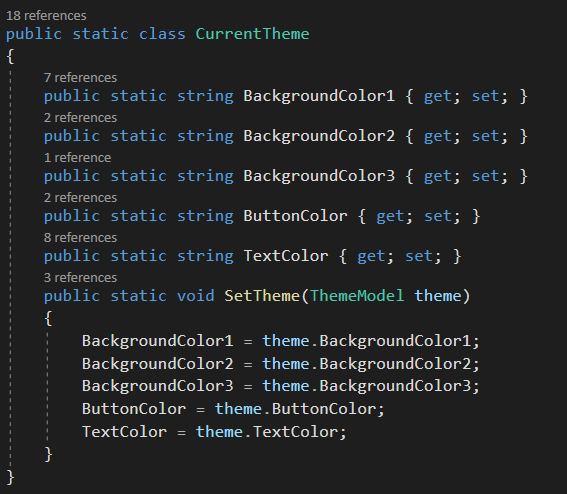
\includegraphics[width=10cm]{rys/gitchanges4.2.13.png}
			\caption{Klasa statyczna przechowująca motyw}
			\label{rys:Klasa statyczna}
		\end{center}
	\end{figure}
\\
	Następnie należało stworzyć metodę inicjalizującą, która ustawia motyw oraz wywołać ją w momencie ładowania aplikacji.
	\begin{figure}[!htb]
		\begin{center}
			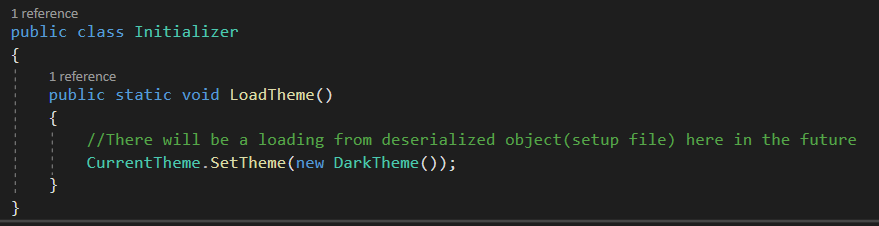
\includegraphics[width=15cm]{rys/gitchanges4.2.14.png}
			\caption{Klasa inicjalizująca}
			\label{rys:Klasa inicjalizująca}
		\end{center}
	\end{figure}
	\begin{figure}[!htb]
		\begin{center}
			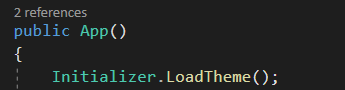
\includegraphics[width=10cm]{rys/gitchanges4.2.15.png}
			\caption{Klasa inicjalizująca - wywołanie}
			\label{rys:Klasa inicjalizująca - wywołanie}
		\end{center}
	\end{figure}
}

\textit
{
\newpage
	Potem należało napisać mechanizm aktualizujący widok po każdym załadowaniu
	\begin{figure}[!htb]
		\begin{center}
			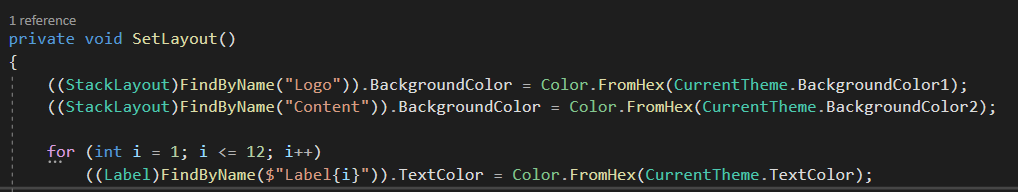
\includegraphics[width=15cm]{rys/gitchanges4.2.16.png}
			\caption{Aktualizacja widoku}
			\label{rys:Aktualizacja widoku}
		\end{center}
	\end{figure}
\\
	Ostatnim krokiem było utworzenie switcha oraz jego mechanizmu działania
	\begin{figure}[!htb]
		\begin{center}
			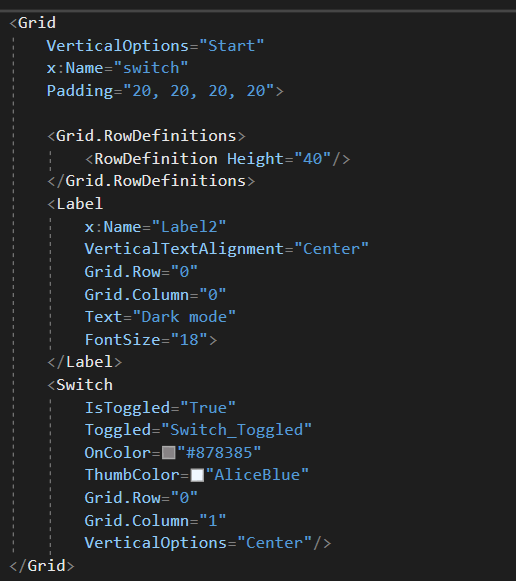
\includegraphics[width=10cm]{rys/gitchanges4.2.17.png}
			\caption{Widok XAML dla switcha}
			\label{rys:Widok XAML dla switcha}
		\end{center}
	\end{figure}
	\begin{figure}[!htb]
		\begin{center}
			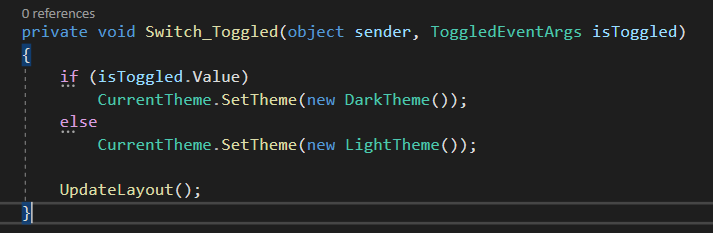
\includegraphics[width=15cm]{rys/gitchanges4.2.18.png}
			\caption{Mechanizm działania switcha}
			\label{rys:Mechanizm działania switcha}
		\end{center}
	\end{figure}
}

\newpage
\textit
{
	Efekt finalny:
	\begin{figure}[!htb]
		\begin{center}
			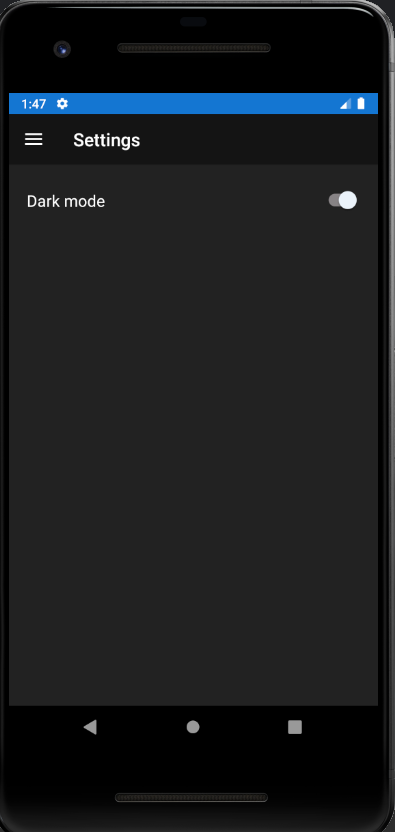
\includegraphics[width=6cm]{rys/gitchanges4.2.19.png}
			\caption{Dark mode włączony}
			\label{rys:Dark mode włączony}
		\end{center}
	\end{figure}
\\
	\begin{figure}[!htb]
		\begin{center}
			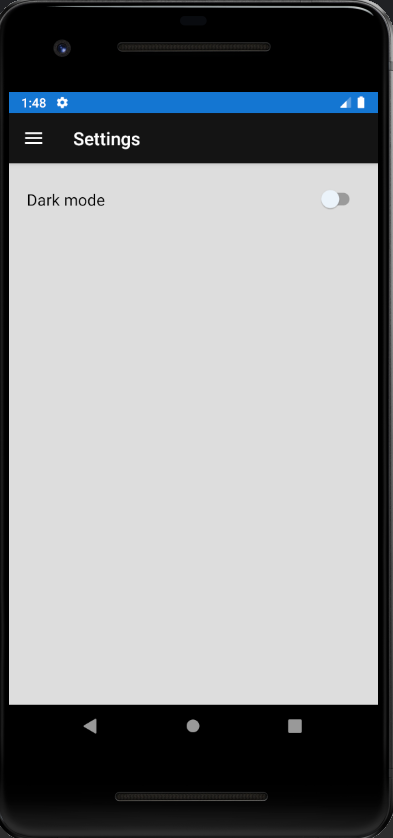
\includegraphics[width=6cm]{rys/gitchanges4.2.20.png}
			\caption{Dark mode wyłączony}
			\label{rys:Dark mode wyłączony}
		\end{center}
	\end{figure}
}



